\newpage
\section{Introducción}

	Desde la aparición de las primeras fotografías, las personas han buscado ``inmortalizar'' escenas, objetos o personas, con el objetivo de, en el área de las ciencias, extraer información útil de las mismas que pueda ser utilizada para su análisis o estudio. Con el surgimiento de los primeros formatos digitales, la necesidad pasó por encontrar métodos automáticos que permitieran clasificar y reconocer elementos dentro de las imágenes. Desde reconocer texto manuscrito, texto en carteles publicitarios y patentes, hasta identificar personas, animales y zonas con agua en una imagen satelital. La cantidad de potenciales aplicaciones que se pueden obtener es enorme. Es por eso que en campos de investigación como visión por computadora, este es un tema de interés. Sin embargo, la clasificación en imágenes naturales no es una tarea para nada sencilla. Por ejemplo, en el reconocimiento de texto, las imágenes naturales contienen mucha información ``extra'' que se tiene que tener en cuenta. Ya sea la existencia de otros objetos ajenos a la clasificación, es decir, elementos que no son texto como así también variaciones propias en las características de la misma imagen.
	
	Hoy en día se ha avanzado mucho en el área de la clasificación en escenas naturales. Se han desarrollado muchas aplicaciones como aquellas capaces de reconocer personas \cite{DT05}, patentes de vehículos \cite{DAB}, entre otros. Si bien, dichos avances muestran que es posible realizar lo mismo en algunos ámbitos, en otros como el reconocimiento de texto sigue siendo un desafío.
	
	\subsection{El problema}

	La gran cantidad de imágenes y documentos existentes en la actualidad ha motivado el desarrollo de modelos y métodos robustos para la búsqueda automatizada de información con el objeto de reducir los problemas asociados a su análisis e interpretación. La extracción y reconocimiento de texto en imágenes naturales, es decir, imágenes de escenas de la vida diaria y/o adquiridas en condiciones no controladas, es un problema de gran interés tanto desde el punto de vista teórico como del de las aplicaciones.  Sin embargo, a diferencia del problema de reconocimiento de texto en documentos escaneados, el reconocimiento de texto en imágenes naturales plantea problemas difíciles de abordar mediante el uso de técnicas tradicionales basadas en OCR (\textit{Optical Character Recognition}, por su denominación en inglés). Esto resulta evidente si se consideran los cambios en la iluminación, los distintos puntos de vista, las diferentes tipografías, estilos, etc. que se ven reflejadas en imágenes de la vida cotidiana.
	
			\begin{figure}[htbp]
				\centering
				\centerline{
					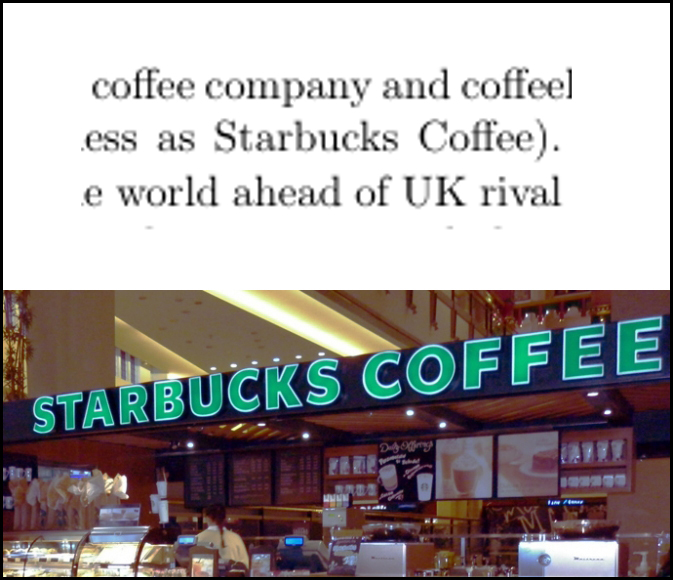
\includegraphics[scale=0.31]{img/ocr_vs_naturalImg_3.jpg}
				}
				\caption[OCRvsNaturales]{La parte superior muestra la imagen de un texto representada con una fuente de computadora donde se puede observar las palabras ``Starbucks Coffee''. La parte inferior expone las mismas palabras pero en una escena natural. Esto se realiza con el objetivo de observar las diferencias que hay entre analizar texto simple (fuente de computadora) y realizar el mismo trabajo en una imagen real}
				\label{fig: Optophone}
			\end{figure}
			
	En la literatura, uno de los esquemas de procesamiento más utilizados ha sido la detección de regiones dentro la imagen que corresponden a texto, su rectificación y la posterior aplicación de técnicas estándar de OCR (Kumar et al., 2007). Sin embargo, esta clase de técnicas se encuentra limitada a los escenarios en donde el OCR funciona correctamente, p.ej. en el reconocimiento de texto impreso (De Campos et al., 2009).

	Recientemente, se propuso un modelo (Wang et al., 2011) que emplea un esquema basado en técnicas de reconocimiento conocidas de la literatura de \textit{reconocimiento de objetos} (Navneet Dalal et al., 2005). En este caso, cada carácter alfanumérico se considera como un objeto a detectar y, empleando un conjunto de muestras de entrenamiento, se genera un modelo de clasificación mediante técnicas de aprendizaje supervisado (Christopher M. Bishop, 2007). Dada una nueva imagen, cada uno de estos clasificadores genera un conjunto de hipótesis sobre la presencia (y su ubicación) de cada símbolo alfanumérico en particular. Estas detecciones se utilizan luego en la detección de palabras específicas a partir de un léxico predefinido. Una particularidad del modelo propuesto por Wang et. al es la utilización de imágenes \textit{sintéticas} (generadas mediante simulación) en la generación de muestras de entrenamiento. Este enfoque reduce el problema de tener que recolectar una gran cantidad de imágenes naturales lo cual consume tiempo y esfuerzo. Mediante diferentes tipos de transformaciones, se busca crear un conjunto de imágenes de caracteres lo más parecido posible a uno real.
	
	
	\subsection{Sobre el trabajo}

	Esta tesis presenta una reimplementación de una sección del trabajo presentado por Wang et. al. en \cite{wang}. En dicha sección, los autores buscan establecer un método para poder reconocer caracteres en imágenes naturales. Para esto proponen usar un clasificador llamado \textit{Random Ferns} (se explica en detalle en el próximo capítulo) para lograr este objetivo.
	
	Este trabajo tiene como finalidad analizar la performance en el reconocimiento de caracteres en imágenes naturales de dicho clasificador. Esto se realiza a través de diferentes experimentos que buscan evaluar diferentes conjuntos de imágenes. El primero es usando imágenes reales, de la misma manera que Wang et. al., con lo cual se busca comparar ambas implementaciones. Posteriormente, se busca analizar como influyen los caracteres sintéticos o fuentes en diferentes proporciones. Estas se alteran con el objetivo de intentar imitar a las imágenes reales y ver si se puede alcanzar o superar los resultados del primer conjunto. Por último y a diferencia de los autores originales, se propone entrenar al clasificador con  un conjunto nuevo que surge de mezclar en diferentes proporciones imágenes reales y sintéticas.

	\subsection{Trabajos Relacionados}
	
	Se han propuesto muchos enfoques para afrontar el problema del reconocimiento de texto en imágenes naturales. De Campos et al. en \cite{dCBV09} comparan la performance de varios clasificadores (dentro de los cuales hay un motor de OCR comercial\footnote{http://abbyy.com/finereader}) sobre un dataset que ellos mismos crearon llamado \textit{Chars74K}. Sobre este dataset se corren varios experimentos del presente trabajo. Las conclusiones del trabajo destacan la dificultad que tienen los motores de OCR al momento de clasificar caracteres en imágenes naturales. Además, remarcan los beneficios de usar datos sintéticos para el entrenamiento los cuales logran un porcentaje de reconocimiento muy similar al obtenido con imágenes reales. También, realizan experimentos sobre un conjunto de imágenes de caracteres manuscritos. Sin embargo, no logran obtener buenos resultados en comparación con los otros experimentos. 
	
	Otro enfoque lo proponen B. Gatos et al. en \cite{GPP03}. El mismo consiste en una nueva metodología que ayuda a la detección, la segmentación y el reconocimiento automático de texto en imágenes naturales. Básicamente, la metodología consiste en lograr una eficiente binarización de las imágenes naturales. Para esto, dada una imagen natural, generan dos imágenes nuevas a partir de la original. La primera es una representación en escala de grises y la segunda es la versión invertida de la primera. Posteriormente, se les aplican diferentes técnicas para mejorarlas y así obtener la imagen binaria. Luego utilizan una función de decisión para elegir qué imagen contiene información de texto y a dicha imagen se le realiza un post-procesamiento para eliminar el ruido existente y mejorar su calidad. Después se realiza la detección de las áreas que contienen texto para poder utilizar finalmente el motor de OCR. Uno de los problemas que se desprenden de este enfoque es que al depender de un motor de OCR, el procesamiento que se realiza a la imagen tiene que ser muy bueno ya que la mayoría de las imágenes contienen ciertos defectos como una pobre iluminación, falta de foco, entre otros.

	L. Neumann y J. Matas \cite{LNJM} se diferencian de los enfoques tradicionales que constan en varias etapas de procesamiento y lo reemplazan con un marco de trabajo que consta de la verificación de hipótesis procesando de manera simultánea múltiples líneas de texto. Además, usan fuente de computadora como conjunto de entrenamiento.
	
	
	\subsection{Estructura de la Tesis}

	Esta tesis se desarrolla a lo largo de 5 capítulos.	
		
	En el capítulo 2 se procede a explicar los conceptos teóricos que involucran el presente trabajo. Principalmente se abordan los principios básicos del aprendizaje supervisado. Posteriormente se describen los conceptos necesarios para poder introducir  el clasificador Random Ferns. Finalmente, se realiza una introducción a las nociones básicas del procesamiento de imágenes.
	
	 En el capítulo 3, se describe el trabajo realizado por Wang et al. en \cite{wang} y se explica qué partes del mismo se han implementado en la presente tesis.

	En el capítulo 4, se abordan los experimentos realizados en el trabajo. Se describe tanto la implemetación del pipeline de procesamiento, como así también su diseño, el dataset usado y los resultados obtenidos. Por último se realiza un análisis completo de los resultados.
	
	En el último capítulo, de conclusiones y trabajos futuros, se hace un resumen de lo logrado a lo largo de esta tesis así como un descripción de los objetivos futuros que se pretenden seguir en este trabajo.

	
	%\subsection{Sobre Reconocimiento óptico de caracteres}

	\subsubsection{Definición del problema}
	
	El reconocimiento óptico de caracteres, usualmente abreviado OCR(por sus siglas en inglés), es la conversión mecánica o electrónica de imágenes escaneadas de texto impreso o mecanografiado en texto que pueda ser interpretado por una computadora. Es ampliamente utilizado como una forma de entrada de datos de algún tipo de fuente de datos original en papel, así sean documentos de pasaportes, facturas, extractos bancarios, recibos, tarjetas de visita, correo, o cualquier número de registros impresos\cite{arh-passport}\cite{arh-card}. Es un método común para la digitalización de textos impresos que pueden ser electrónicamente editados, buscados, almacenados de manera compacta, expuestos en linea y usados en procesos de máquinas como traducción de máquina, texto a voz, extracción de datos y minería de texto\cite{gbook}\cite{creaceed}. OCR es un campo de investigación en reconocimiento de patrones, inteligencia artificial y visión por computadora.
	
	\subsubsection{Aplicaciones}
		\begin{itemize}
			\item Reconocimiento automático de patentes\cite{arh-anpr}.
			\item Extraer información de una tarjeta de negocio a una lista de contacto \cite{x-root}.
			\item Hacer posible la búsqueda de imágenes electrónicas de documentos impresos. ej: \textit{Google Books} \cite{gbook}
			\item Convertir la escritura manual en tiempo real para controlar una computadora (\textit{pen computing})\cite{GKurt}\cite{sunnyside}.
			\item Tecnología de asistencia para usuarios ciegos y con deficiencias visuales \cite{creaceed}.
		\end{itemize}	
		
	\subsubsection{Componentes de un sistema OCR}
	
	A continuación se presentaran las diferentes etapas de un sistema OCR, como se puede apreciar en la figura \ref{fig: Sistema OCR}. Esta sección tiene como objetivo mostrar un panorama general de como funciona un sistema OCR, no tiene como objetivo adentrarse en detalles de implementación. En cada etapa se procederá a explicar brevemente cuales son las características importantes, haciendo incapié en la etapas de extracción de características y en la de clasificación y reconocimiento dado que son las etapas que se abordaron en este trabajo.
	
		\begin{figure}[htbp]
			\centering
			\fbox{ 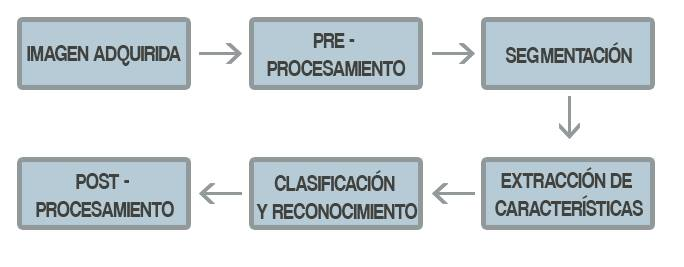
\includegraphics[scale=0.4]{img/OCR_pipeline_1.jpg} }
			\caption{Pipeline de un sistema OCR.}
			\label{fig: Sistema OCR}
		\end{figure}
	
		\paragraph{Pre-procesamiento} ~\\

		 El software de OCR aveces realiza un pre-procesamiento de las imágenes con el objetivo de tener más chances de un reconocimiento exitoso. Estas técnicas incluyen:
		  \begin{itemize}
		  	\item \textit{Enderezar} - Si el documento no está alineado debidamente cuando se escanea, puede necesitar posteriormente que se rote unos pocos grados en sentido horario o anti-horario con el objetivo de mantener el texto perfectamente vertical u horizontal \ref{fig: Enderezar}.
		  	\item \textit{Quitar manchas} - remover puntos negativos  y positivos, suavizar los bordes \ref{fig: Imagen con particulas} \ref{fig: Imagen suavizada}.
		  	\item \textit{Binarización} - Convertir la imagen de color o en escala de grises a blanco y negro (se llama "imagen binaria" justamente porque hay dos colores solamente). En algunos casos, esto es necesario para el algoritmo de reconocimiento de caracteres; en otros casos esta etapa se omite dado que el algoritmo tiene un mejor rendimiento con la imagen original \ref{fig: Binarizacion}.
		  	\item \textit{Eliminación de lineas} - Limpia las lineas y las cajas sin glifo \ref{fig: Eliminacion de lineas}.
		  	\item \textit{Análisis de disposición o "zoning"} - Identifica columnas, párrafos, títulos, etc. como bloques diferentes. Especialmente importante en tablas o disposiciones multi-columna \ref{fig: Zoning}.
		  	\item \textit{Detección de lineas y palabras} - Establece  la base para la forma del caracter y la palabra, separa las palabras si es necesario.
		  	\item \textit{Segmentación o aislación de caracter} - Múltiples caracteres que están conectados debido a artefactos de imagen deben ser separados; caracteres individuales que son separados en multiples piezas debido a artefactos deben ser conectados \ref{fig: Segmentacion}.
		  	\item \textit{Normalización de escala y relación de aspecto \ref{fig: Normalizacion y Suavizado}.}
		  \end{itemize}
		  
		\begin{figure}[htbp]
			\centering
			\subfloat[Imagen original torcida\label{fig: Imagen torcida}]{
				\fbox{ 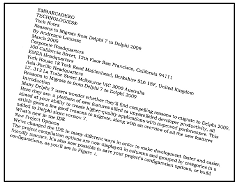
\includegraphics[scale=0.7]{img/skew_img.png} }
			}
			\subfloat[Imagen enderezada\label{fig: Imagen destorcida}]{
				\fbox{ 
\includegraphics[scale=0.7]{img/deskew_img.png} }
			}
			\caption{Imagen enderezada}
			\label{fig: Enderezar}
		\end{figure}	
			  
		\begin{figure}[htbp]
			\centering
			\fbox{ 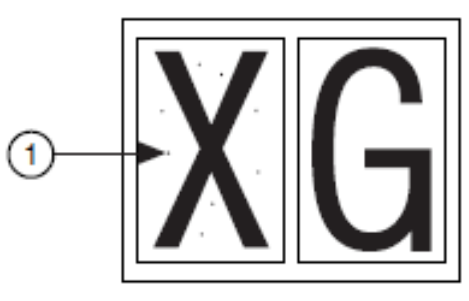
\includegraphics[scale=0.4]{img/rem_particles.png} }
			\caption[Imagen con partículas]{Comparación de caracteres con y sin partículas. 1. Imagen con partículas.}
			\label{fig: Imagen con particulas}
		\end{figure}
		
		\begin{figure}[htbp]
			\centering
			\fbox{ 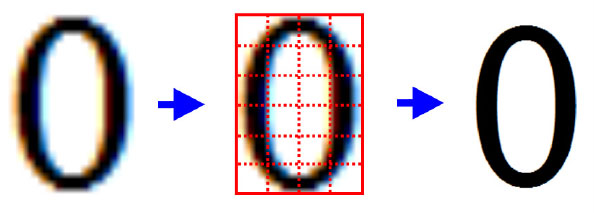
\includegraphics[scale=0.4]{img/smooth_char.png} }
			\caption{Imagen suavizada.}
			\label{fig: Imagen suavizada}
		\end{figure}
		
		\begin{figure}[htbp]
			\centering
			\subfloat[Imagen Original\label{fig: Imagen bin original}]{
				\fbox{ 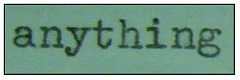
\includegraphics[scale=0.7]{img/bin_1.png} }
			}
			\subfloat[Imagen binarizada\label{fig: Imagen binarizada}]{
				\fbox{ 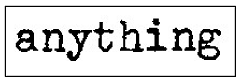
\includegraphics[scale=0.7]{img/bin_2.png} }
			}
			\caption{Binarización de una imagen}
			\label{fig: Binarizacion}
		\end{figure}
		
		\begin{figure}[htbp]
			\centering
			\subfloat[Imagen Original\label{fig: Imagen lines original}]{
				\fbox{ 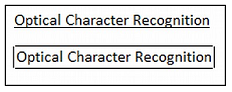
\includegraphics[scale=0.7]{img/lines_1.png} }
			}
			\subfloat[Imagen con las lineas removidas\label{fig: Imagen sin lineas}]{
				\fbox{ 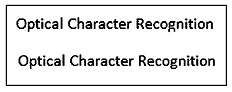
\includegraphics[scale=0.7]{img/lines_2.png} }
			}
			\caption{Eliminación de lineas}
			\label{fig: Eliminacion de lineas}
		\end{figure}
		
		\begin{figure}[htbp]
			\centering
			\fbox{ 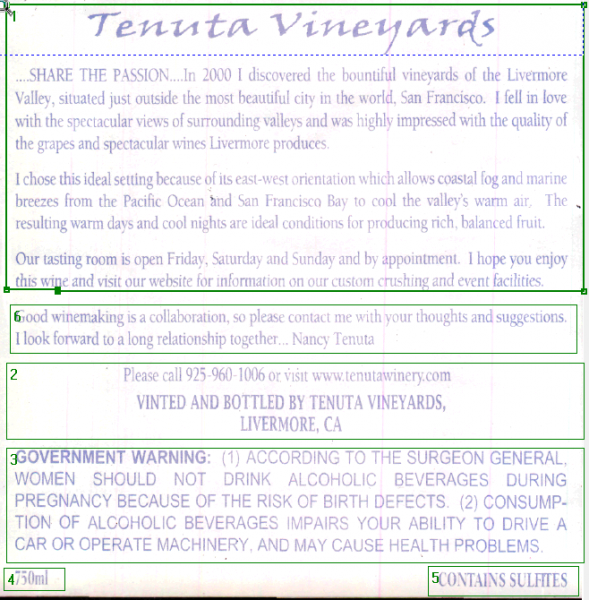
\includegraphics[scale=0.3]{img/zoning.png} }
			\caption{Análisis de disposición o "zoning".}
			\label{fig: Zoning}
		\end{figure}

		\begin{figure}[htbp]
			\centering
			\fbox{ 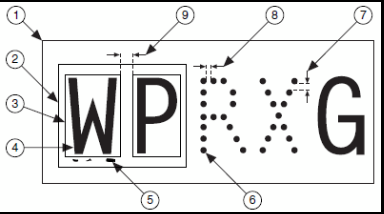
\includegraphics[scale=0.5]{img/segmentation.png} }
			\caption[Segmentación]{Segmentación. 1.Imagen Adquirida, 2.Región de interés, 3.Rectángulo del límite del carácter, 4.Carácter, 5.Artefacto, 6.Elemento, 7.Espaciado vertical, 8.Espaciado horizontal, 9.Espaciado del carácter.}
			\label{fig: Segmentacion}
		\end{figure}
		
		\begin{figure}[htbp]
			\centering
			\fbox{ 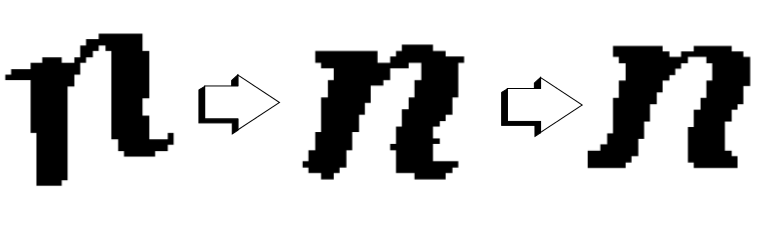
\includegraphics[scale=0.4]{img/norm_and_smoothing.png} }
			\caption{Normalización y suavizado de un símbolo.}
			\label{fig: Normalizacion y Suavizado}
		\end{figure}
	
\newpage
		\paragraph{Ubicación y segmentación}	 ~\\
		
		La segmentación es el proceso que determina los componentes de una imagen. Es necesario ubicar las regiones del documento donde se han impreso los datos y distinguirlos de los gráficos y las figuras. Por ejemplo, cuando se realiza el ordenamiento de correo automático, la dirección debe estar localizada y separada de otras impresiones en el sobre como las estampillas o logos de empresa, anterior al reconocimiento.
		
		Aplicado al texto, la segmentación es la aislación de caracteres o palabras. La mayoría de los algoritmos de reconocimiento óptico de caracteres segmentan las palabras en caracteres aislados los cuales son reconocidos individualmente. Usualmente esta segmentación es realizada aislando cada componente conectado, es decir, cada área negra conectada. Esta técnica es fácil de aplicar, pero los problemas ocurren si los caracteres se tocan o si los caracteres están fragmentados y consisten de varias partes, si el texto tiene mucho ruido o se confunde con alguna imagen, entre otros. ~\ref{fig: Caracter quebrado}~\ref{fig: Caracteres unidos 1}~\ref{fig: Caracteres unidos 2}~\ref{fig: Caracteres en graffiti}~\ref{fig: Captcha}.

		\begin{figure}[htbp]
			\begin{minipage}{.3\linewidth}
				\centering
				\subfloat[Captcha\label{fig: Captcha}]{
					\fbox{ 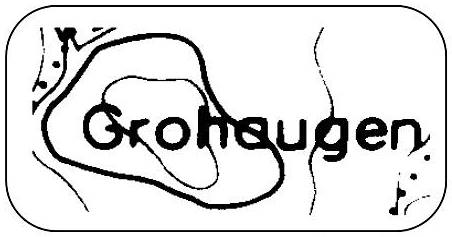
\includegraphics[scale=0.2]{img/degraded_1.jpg} }
				}
			\end{minipage}
			\begin{minipage}{.3\linewidth}
				\centering
				\subfloat[Carácter quebrado\label{fig: Caracter quebrado}]{
					\fbox{ 
\includegraphics[scale=0.3]{img/degraded_2.jpg} }
				}
			\end{minipage}
			\begin{minipage}{.3\linewidth}
				\centering
				\subfloat[Caracteres unidos por la tipografía\label{fig: Caracteres unidos 1}]{
					\fbox{ 
\includegraphics[scale=0.3]{img/degraded_3.jpg} }
				}
			\end{minipage}
			\begin{minipage}{.3\linewidth}
				\centering
				\subfloat[Carácter con linea superpuesta\label{fig: Caracter y linea}]{
					\fbox{ 
\includegraphics[scale=0.3]{img/degraded_4.jpg} }
				}
			\end{minipage}
			\begin{minipage}{.3\linewidth}
				\centering
				\subfloat[Caracteres unidos\label{fig: Caracteres unidos 2}]{
					\fbox{ 
\includegraphics[scale=0.3]{img/degraded_5.jpg} }
				}
			\end{minipage}
			\begin{minipage}{.3\linewidth}
				\centering
				\subfloat[Un graffiti como el de la imagen puede hacer pasar el texto como imagen.\label{fig: Caracteres en graffiti}]{
					\fbox{ 
\includegraphics[scale=0.2]{img/text_like_graphic.jpg} }
				}
			\end{minipage}
			\caption{Problemas de segmentación}
			\label{fig: Problemas de segmentacion}
		\end{figure}
		
	
		\paragraph{Extracción de características} ~\\
		
		El objetivo de la extracción de características es capturar los rasgos esenciales de los caracteres para formar vectores de características y es generalmente aceptado como uno de los problemas más difíciles en el reconocimiento de patrones. Se vuelve sencillo para el clasificador el clasificar entre clases diferentes teniendo en cuenta estas características \cite{PSH2011}. Acorde al trabajo de C. Y. Suen \cite{Suen86}, los rasgos de un carácter pueden ser clasificados en dos clases: características globales o estadísticas y características estructurales o topológicas.
		\begin{itemize}
			\item \textbf{Características globales o estadísticas}. \\
				Las características globales son obtenidas del arreglo de puntos que constituyen la matriz del carácter. Estas características pueden ser detectadas fácilmente en comparación con las características topológicas. Además no son afectadas demasiado por el ruido o la distorción en comparación a las topológicas. Un número de técnicas se utilizan para lograr la extración de características, estas son: \textit{momentos, zonificación, histogramas de proyección, n-tuplas y cruce y distancias}
				\begin{itemize}
					\item \textbf{Momentos}
					En este caso los diferentes puntos presentes en un carácter son utilizados como características. Heutte et al. \cite{Heutte98} decían que estos métodos son más comúnmente usados en el reconocimiento de caracteres.
					\item \textbf{Zonificación}
					De acuerdo con esta técnica, la matriz del carácter es dividida en pequeñas porciones o zonas. Las densidades de los píxeles en cada zona son calculadas y usadas como características. Este concepto fue sugerido por Hussain et al.\cite{Hussain72}.
					\item \textbf{Histogramas de proyección}
					Los histogramas de proyección nos da el número de píxeles negros en las direcciones horizontal y vertical de un área específica del carácter. El concepto fue introducido por M. H. Glauberman \cite{Glauberman56}. Los histogramas de proyección pueden ser vertical, horizontal, diagonal izquierda o derecha.
					\item \textbf{N-tuplas}
					De acuerdo con este método, la posición de los píxeles blancos o negros en la imagen de un carácter es considerado una característica. El método fue desarrollado por Tarling y Rohwer \cite{TR93}.
				\end{itemize}
			\item \textbf{Características estructurales o topológicas}. \\
				Estas características están relacionadas con la geometría del conjunto de caracteres. Algunas de estas características son concavidades y convexidades en los caracteres, el número de puntos finales, el número de agujeros en los caracteres, etc. Muchas investigaciones fueron realizadas con el objetivo de encontrar diferentes características estructurales.
				
				Rocha y Pavlidis \cite{RP94} propusieron un método para el reconocimiento de caracteres impresos del tipo multi-fuente. Para este método se han utilizado características estructurales tales como puntos singulares, arcos convexos y trazos.
				
				Otro método similar fue propuesto por A. Amin \cite{Amin2000}. Aquí se han usado características estructurales como el número de subpalabras, el número de picos en cada subpalabra, el número de curvas de cada pico, entre otros.
				
		\end{itemize}
		  
		  	En el presente trabajo, las características de una imagen son representadas por un vector binario que se obtiene de binarizar el descriptor HOG(concepto descripto en la sección \ref{sec: HOG}) de dicha imagen con un umbral pre-calculado. Este método de extracción de características se abordará más adelante en el capítulo 4 cuando se explique el pipeline de procesamiento.
	  
		\paragraph{Clasificación y Reconocimiento} ~\\
		
		La clasificación es el proceso de identificar cada carácter y asignarle la clase correcta. La clasificación se hace generalmente mediante la comparación de los vectores de características que corresponden al carácter de entrada con el representante de cada clase de carácter. Pero antes de hacer esto, el clasificador debe entrenarse con un conjunto de entrenamiento que represente a las diferentes clases de caracteres. Varios investigadores han propuesto métodos de clasificación dentro de los cuales se encuentran los métodos estadísticos, métodos sintácticos, comparación de plantillas, redes neuronales artificiales, métodos de núcleo~\cite{NNSJ}~\cite{SA96}~\cite{RYVY2010}.
		
		Como se procederá a explicar en detalle en el capítulo 3, el clasificador que se usa en este trabajo es Random Ferns. Las razones de su elección se basan en que es un clasificador multi-clase bastante eficiente y dado que el problema en cuestión es clasificar caracteres (representan 62 clases en total), su elección resulta apropiada.
		
		El aporte de este trabajo se basa en analizar la performance del clasificador Random Ferns cuando es entrenado con caracteres sintéticos. Si bien este enfoque fue abordado en \cite{wang}, en dicho trabajo no se puede apreciar como influye en la clasificación la cantidad de imágenes sintéticas usadas al entrenar el clasificador. En su trabajo, hacen uso de 1000 imágenes sintéticas por clase para entrenar el clasificador y realizan una comparación de performance entre el entrenamiento con imágenes sintéticas y el realizado con imágenes reales. Este trabajo va un paso más allá y busca ver si el número de imágenes sintéticas por clase influye realmente en la performance y además se busca analizar un nuevo enfoque en el cual se mezclan en diferentes proporciones imágenes reales con sintéticas para observar que tan efectivo resulta ser el clasificador en esas condiciones.
		
		\paragraph{Post-procesamiento} ~\\
		
		La precisión de OCR puede ser incrementada si la salida está restringida por un lexicón, que es una lista de palabras cuya aparición está permitida dentro del documento. Este puede ser, por ejemplo, todas las palabras del lenguaje español, o un lexicón mas técnico para un campo en particular. Esta técnica puede ser problematica si el documento contiene palabras que no están en el lexicón, como nombres propios.
		
		La salida puede ser texto plano o un archivo de caracteres, pero sistemas de OCR más sofisticados pueden conservar la disposición original de la pagina y producir, por ejemplo, un PDF con anotaciones que incluyan la imagen original de la página y una representación textual de búsqueda.
		
		Conocer la gramática del lenguaje que está siendo escaneado puede ayudar a determinar si la palabra es un verbo o un sustantivo, por ejemplo, permitiendo una gran precisión.
		
	\subsubsection{Errores típicos en OCR}
	
		La precisión de los sistemas de OCR es, en la práctica, directamente dependiente de la calidad de los documentos de entrada. Las principales dificultades se pueden clasificar como sigue:
		\begin{itemize}
			\item \textit{Variaciones en la forma}, debido a las variaciones en el estilo y los remates o serifas.
			\item \textit{Deformaciones}, causados por caracteres quebrados, manchados y moteados.
			\item \textit{Variación en el espaciado}, debido a los superíndices, subíndices, sesgo y la variable de espaciado.
			\item \textit{Mezcla de texto e imágenes}.
		\end{itemize}
		Estas imperfeccciones pueden afectar y ocasionar problemas las diferentes etapas del proceso de reconocimiento de un sistema OCR, resultando en errores de clasificación y rechazos.	
	
		

	
	%	\newpage
	\subsection{Repercusión social del tema}
		\label{sec:repercusion_social}
		Cheap brainstorm:
		\begin{itemize}
		 \item digitalizar documentos
		 \item brindar mejor calidad de  vida a gente con discapacidades
		 
		\end{itemize}


